\documentclass[11pt,a4paper]{article}

\usepackage[utf8]{inputenc}
\usepackage[T1]{fontenc}
\usepackage{amsmath,amssymb,amsfonts}
\usepackage{booktabs}
\usepackage{geometry}
\usepackage{hyperref}
\usepackage{siunitx}
\usepackage{float}
\usepackage{graphicx}
\usepackage{xcolor}
\usepackage{longtable}

\geometry{margin=1in}

\title{QoI-Preserving Lossy Compression for SAM3D Turbulence Data}

\begin{document}

\maketitle

\begin{abstract}
We have applied Quantity-of-Interest (QoI) preserving lossy compression to SAM3D Large-Eddy Simulation (LES) data from the LASSO-ENA project. 
Given 6 initial 3D data arrays and 9 derived QoI data arrays, we bound all 15 arrays with sepecified relative error bound only by compressing the 6 initial arrays with certain error bound.
The 9 QoIs we consider include 5 bilinear QOIs, 3 quadratic variances, and 1 higher-order skewness.
Since QPET fails when one initial data point is used to derive multiple QoI data points and it does not support bounding multiple QoIs, we only adopted its method to calculate point-wise error bound when compressing initial data arrays.
While we successfully bound all initial arrays and QoI arrays, the overall compression ratio is relatively low(8.5x) even we used a loose error bound(1e-2). We further introduce an empirical per-field binary-search framework supporting SZ3, zfp, and SPERR that substantially improves the compression ratio (up to $30.5\times$ with SZ3 at $\tau=10^{-2}$) while still bounding all nine QoIs.
\end{abstract}


%==============================================================================
\section{Data Overview}
%==============================================================================

The data originates from the LASSO-ENA (Large-Eddy Simulation ARM Symbiotic Simulation and Observation -- Eastern North Atlantic) project, using the SAM (System for Atmospheric Modeling) model v6.10.3 with LASSO modifications.

Six 3D variables are used for compression, each with shape $(N_z, N_y, N_x) = (260, 256, 256)$ and dtype \texttt{float32}:

\begin{table}[H]
\centering
\caption{Primary 3D Variables for Compression}
\begin{tabular}{llll}
\toprule
\textbf{Variable} & \textbf{Description} & \textbf{Units} & \textbf{Typical Range} \\
\midrule
$U$ & Zonal wind component & m/s & 3 -- 19 \\
$V$ & Meridional wind component & m/s & $-22$ -- $-3$ \\
$W$ & Vertical wind component & m/s & $-0.27$ -- 0.31 \\
$PP$ & Pressure perturbation & Pa & $-0.72$ -- 0.84 \\
$TABS$ & Absolute temperature & K & 240 -- 287 \\
$QV$ & Water vapor mixing ratio & g/kg & 0.02 -- 7.9 \\
\bottomrule
\end{tabular}
\end{table}

\noindent\textbf{Total timesteps}: 96

\noindent\textbf{Dimension per array}: $(N_z, N_y, N_x) = (260, 256, 256)$

\noindent\textbf{Memory footprint}: \SI{68.2}{\mega\byte} per variable (float32), \SI{408.9}{\mega\byte} per timestep for 6 variables, \SI{38.4}{\giga\byte} total for 96 timesteps

\begin{figure}[H]
\centering
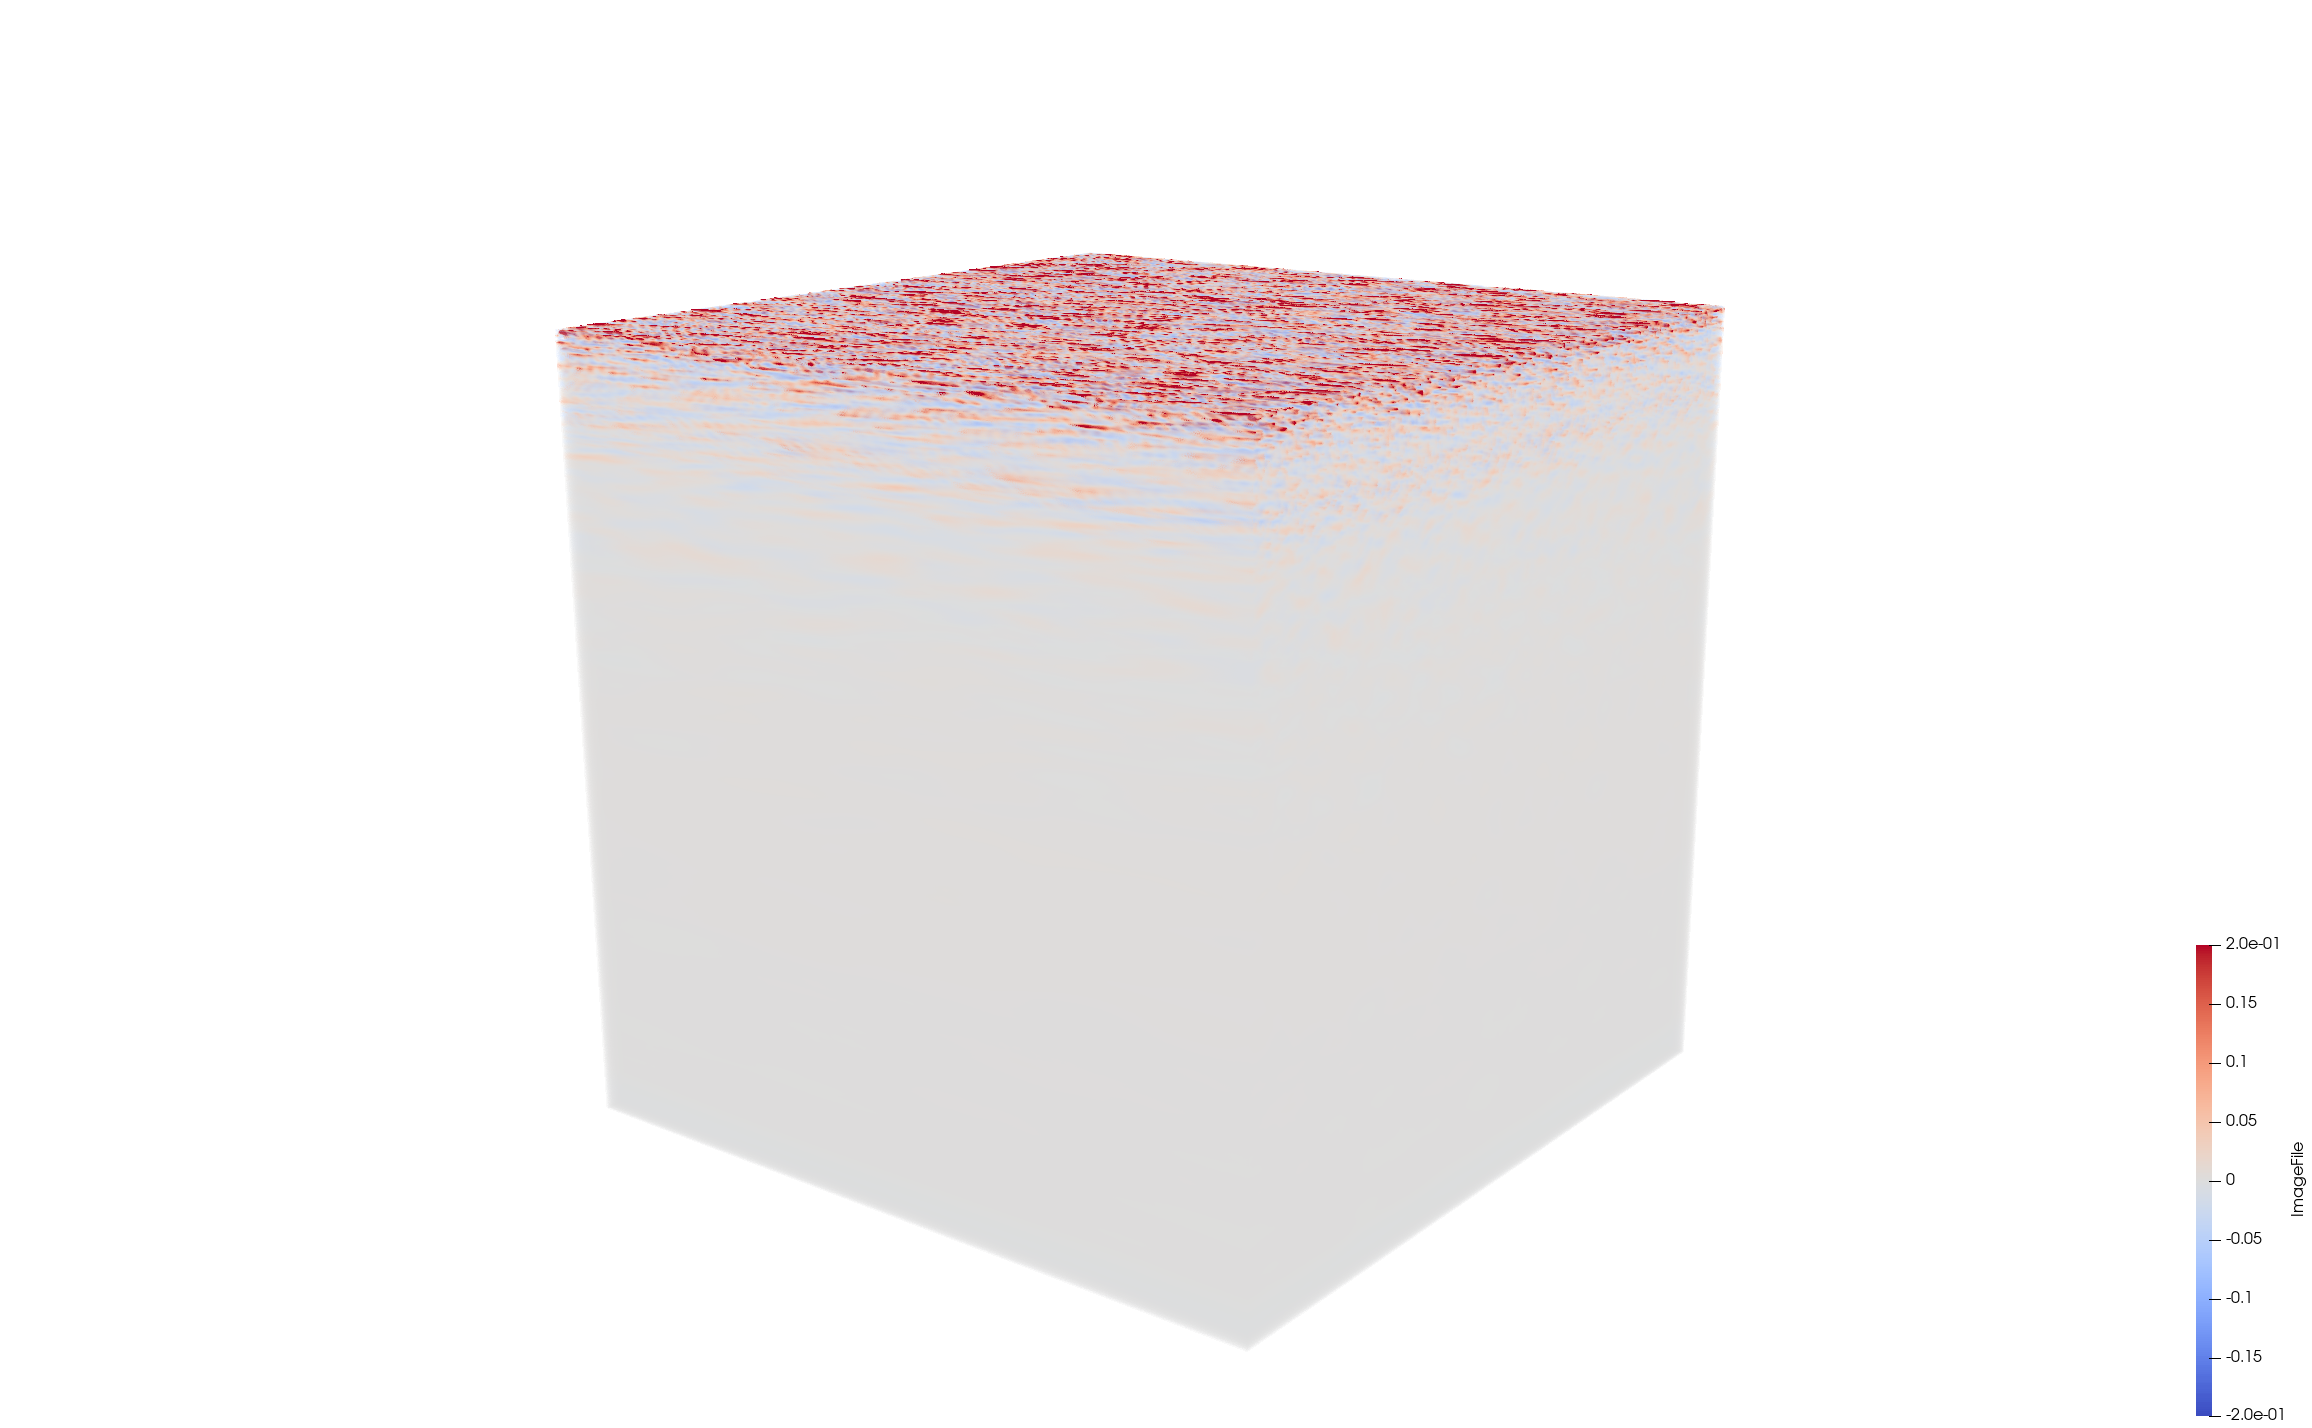
\includegraphics[width=0.8\textwidth]{PP.png}
\caption{Pressure perturbation of time step 1 $(N_z, N_y, N_x)=(260, 256, 256)$}
\end{figure}

\begin{figure}[H]
\centering
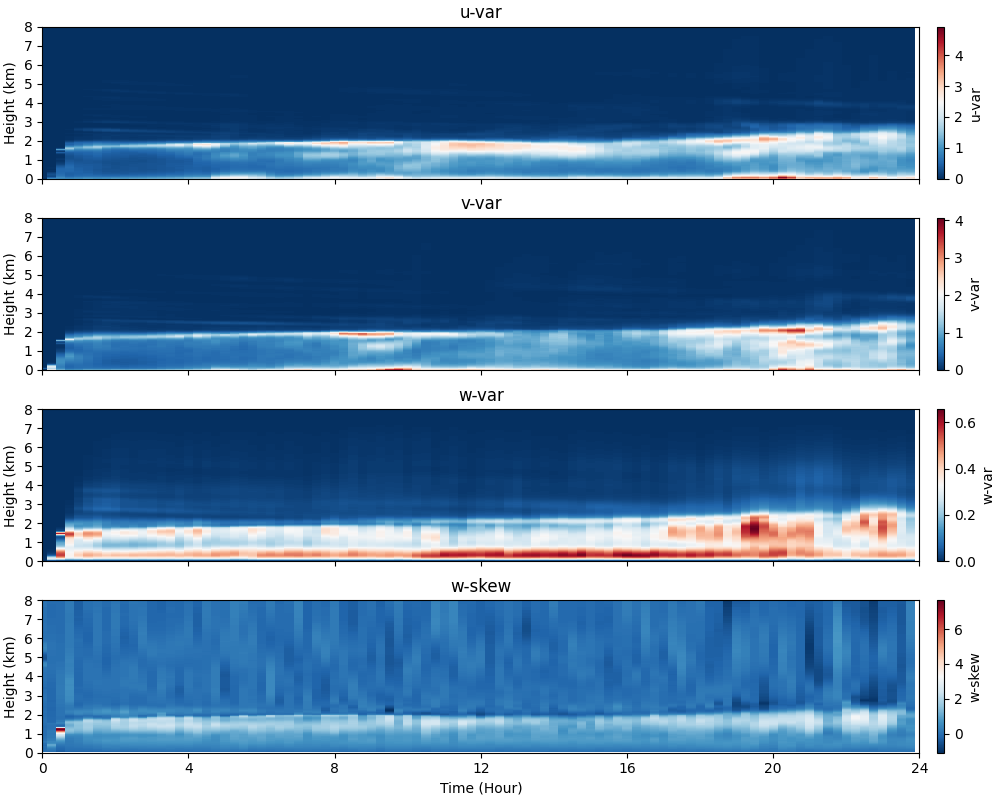
\includegraphics[width=0.9\textwidth]{turbstats.png}
\caption{Turbulence statistics derived from 96 timesteps: velocity variances (uvar, vvar, wvar) and vertical velocity skewness (wskew)}
\end{figure}

%==============================================================================
\section{Quantities of Interest (QoIs)}
%==============================================================================

\subsection{Mathematical Notations}

\begin{table}[H]
\centering
\caption{Symbol Definitions}
\begin{tabular}{ll}
\toprule
\textbf{Symbol} & \textbf{Description} \\
\midrule
$\phi$ & Generic field variable (e.g., $u$, $v$, $w$, $T$, $p$, $q_v$) \\
$\overline{\phi}(z)$ & Horizontal mean of $\phi$ at height $z$ \\
$\phi'$ & Turbulent perturbation ($\phi' = \phi - \overline{\phi}$) \\
$\langle \cdot \rangle_{xy}$ & Horizontal averaging operator over $x$ and $y$ \\
$N_x, N_y, N_z$ & Number of grid points in $x$, $y$, and $z$ directions \\
$\sigma_w(z)$ & Standard deviation of vertical velocity at height $z$ \\
$u', v', w'$ & Perturbations of velocity components \\
$T', p', q_v'$ & Perturbations of temperature, pressure, and water vapor \\
\bottomrule
\end{tabular}
\end{table}

All derived QoIs are based on Reynolds decomposition, separating each field $\phi$ into a horizontal mean and turbulent perturbation:
\begin{equation}
    \phi(x, y, z) = \overline{\phi}(z) + \phi'(x, y, z)
\end{equation}
where the overbar denotes horizontal averaging at each height level:
\begin{equation}
    \overline{\phi}(z) = \langle \phi \rangle_{xy} = \frac{1}{N_x N_y} \sum_{i,j} \phi(x_i, y_j, z)
\end{equation}

The perturbation is computed as:
\begin{equation}
    \phi' = \phi - \langle \phi \rangle_{xy}
\end{equation}

\subsection{Zonal Momentum Flux -- wpup (Bilinear)}
\begin{equation}
    \overline{w'u'}(z) = \langle w'(x,y,z) \cdot u'(x,y,z) \rangle_{xy}
\end{equation}

\subsection{Meridional Momentum Flux -- wpvp (Bilinear)}
\begin{equation}
    \overline{w'v'}(z) = \langle w'(x,y,z) \cdot v'(x,y,z) \rangle_{xy}
\end{equation}

\subsection{Pressure-Velocity Covariance -- wppp (Bilinear)}
\begin{equation}
    \overline{w'p'}(z) = \langle w'(x,y,z) \cdot p'(x,y,z) \rangle_{xy}
\end{equation}

\subsection{Sensible Heat Flux -- wptp (Bilinear)}
\begin{equation}
    \overline{w'T'}(z) = \langle w'(x,y,z) \cdot T'(x,y,z) \rangle_{xy}
\end{equation}

\subsection{Moisture Flux -- wpqvp (Bilinear)}
\begin{equation}
    \overline{w'q_v'}(z) = \langle w'(x,y,z) \cdot q_v'(x,y,z) \rangle_{xy}
\end{equation}

\subsection{Zonal Velocity Variance -- uvar (Quadratic)}
\begin{equation}
    \overline{u'^2}(z) = \langle u'(x,y,z)^2 \rangle_{xy}
\end{equation}

\subsection{Meridional Velocity Variance -- vvar (Quadratic)}
\begin{equation}
    \overline{v'^2}(z) = \langle v'(x,y,z)^2 \rangle_{xy}
\end{equation}

\subsection{Vertical Velocity Variance -- wvar (Quadratic)}
\begin{equation}
    \overline{w'^2}(z) = \langle w'(x,y,z)^2 \rangle_{xy} = \sigma_w^2(z)
\end{equation}

\subsection{Vertical Velocity Skewness -- wskew (Higher-Order)}
\begin{equation}
    S_w(z) = \left\langle \left(\frac{w'}{\sigma_w}\right)^3 \right\rangle_{xy} = \frac{\langle w'^3 \rangle_{xy}}{\sigma_w^3(z)}
\end{equation}
where $\sigma_w(z) = \sqrt{\overline{w'^2}(z)}$ is the standard deviation of vertical velocity at height $z$.

\subsection{Summary of QoIs}

\begin{table}[H]
\centering
\caption{Summary of Quantities of Interest}
\begin{tabular}{llll}
\toprule
\textbf{QoI} & \textbf{Formula} & \textbf{Type} & \textbf{Dependent Fields} \\
\midrule
wpup & $\langle w'u' \rangle_{xy}$ & Bilinear & $W$, $U$ \\
wpvp & $\langle w'v' \rangle_{xy}$ & Bilinear & $W$, $V$ \\
wppp & $\langle w'p' \rangle_{xy}$ & Bilinear & $W$, $PP$ \\
wptp & $\langle w'T' \rangle_{xy}$ & Bilinear & $W$, $TABS$ \\
wpqvp & $\langle w'q_v' \rangle_{xy}$ & Bilinear & $W$, $QV$ \\
uvar & $\langle u'^2 \rangle_{xy}$ & Quadratic & $U$ \\
vvar & $\langle v'^2 \rangle_{xy}$ & Quadratic & $V$ \\
wvar & $\langle w'^2 \rangle_{xy}$ & Quadratic & $W$ \\
wskew & $\langle w'^3 \rangle_{xy} / \sigma_w^3$ & Cubic/Rational & $W$ \\
\bottomrule
\end{tabular}
\end{table}

Note that the $W$ field appears in all 9 QoIs, making it the most constrained field in QoI-preserving compression.

\textcolor{red}{\textbf{Takeaway:} All QoIs are non-trivial functions because they are all non-linear, non operator-separable, and each single data point in the initial data array contributes to multiple QoIs.}

%==============================================================================
\section{Method}
%==============================================================================

\subsection{Input, Output, and Error Bounds}

\textbf{Input files:} Six 3D binary arrays stored as raw float32 files:
\begin{itemize}
    \item \texttt{U\_260x256x256.raw}, \texttt{V\_260x256x256.raw}, \texttt{W\_260x256x256.raw}
    \item \texttt{PP\_260x256x256.raw}, \texttt{TABS\_260x256x256.raw}, \texttt{QV\_260x256x256.raw}
\end{itemize}

\textbf{Input error bounds:} User specifies relative error bounds for:
\begin{itemize}
    \item 6 field arrays: $\epsilon_U, \epsilon_V, \epsilon_W, \epsilon_{PP}, \epsilon_{TABS}, \epsilon_{QV}$
    \item 9 QoI arrays: $\tau_{wpup}, \tau_{wpvp}, \tau_{wppp}, \tau_{wptp}, \tau_{wpqvp}, \tau_{uvar}, \tau_{vvar}, \tau_{wvar}, \tau_{wskew}$
\end{itemize}

\textbf{Output files:} Six SZ3-compressed files with calculated absolute error bounds that satisfy both field and QoI constraints.

\subsection{Point-wise Error Bound Derivation}

Following the QPET framework, for a multivariate QoI function $F(x_1, \ldots, x_n)$ that is not in variable-separated format, we use its first-order Taylor approximation:
\begin{equation}
    F(x'_1, \ldots, x'_n) \approx F(x_1, \ldots, x_n) + \sum_i \frac{\partial F}{\partial x_i}(x_i)(x'_i - x_i)
\end{equation}

This reduces the multivariate QoI to a linear combination format $F = C + \sum_i \alpha_i f(x_i)$ where $\alpha_i = \frac{\partial F}{\partial x_i}$ and $f(x) = x$. The point-wise error bound for each data point is computed using:
\begin{equation}
    t = \frac{T}{\sum_i |\alpha_i|}
\end{equation}
where $T$ is the QoI error threshold. This deterministic bound guarantees that if each point-wise error $|D_i| \leq t$, then $|\sum_i \alpha_i D_i| \leq T$.

\textcolor{red}{\textbf{Takeaway:} Since each single data point in the initial data array contributes to multiple QoIs, the simple edition approach in QPET (which corrects outliers after compression) is not applicable. Instead, we must hard-bound all data points during compression.}

\subsection{Sequential Bound Calculation for Multiple QoIs}

When bounding multiple QoIs that share common input fields, the \textbf{sequence of error bound calculation matters}. Consider our 9 QoIs where the $W$ field appears in all of them:

\textbf{Problem:} The skewness QoI depends on $\sigma_w = \sqrt{\text{wvar}}$, so the wvar error must be known before computing the wskew bound. Similarly, bilinear QoIs like $\langle w'u' \rangle$ need the $W$ bound to allocate the remaining error budget to other fields.

\textbf{Our approach:}
\begin{enumerate}
    \item \textbf{Step 1: Compute wvar bound first.} Since $\text{wvar} = \langle w'^2 \rangle_{xy}$ is quadratic in $W$, we derive:
    \begin{equation}
        \epsilon_W^{wvar} = \frac{\tau_{wvar} \cdot \text{range}(wvar)}{4 \cdot \max_z \langle |w'| \rangle}
    \end{equation}

    \item \textbf{Step 2: Compute wskew bound using known wvar error.} The skewness $S_w = \langle w'^3 \rangle / \sigma_w^3$ has per-datapoint partial derivatives:
    \begin{equation}
        \frac{\partial f_i}{\partial w'_i} = \frac{3(w'_i)^2}{\sigma^3}, \quad \frac{\partial f_i}{\partial(\sigma^2)} = -\frac{3(w'_i)^3}{2\sigma^5}
    \end{equation}
    The $\sigma^2$ term uses the known wvar error from Step 1.

    \item \textbf{Step 3: Compute bilinear QoI bounds.} For $\langle w'\phi' \rangle$, with the $W$ bound already determined, we allocate the remaining error budget to the other field $\phi$:
    \begin{equation}
        \epsilon_\phi = \frac{\tau \cdot \text{range}(QoI) - 2\epsilon_W \cdot \max_z\langle|\phi'|\rangle}{2 \cdot \max_z\langle|w'|\rangle}
    \end{equation}
\end{enumerate}

The final field error bound is the \textbf{minimum} across all QoI-derived bounds:
\begin{equation}
    \epsilon_W = \min(\epsilon_W^{user}, \epsilon_W^{wvar}, \epsilon_W^{wskew}, \epsilon_W^{wpup}, \epsilon_W^{wpvp}, \epsilon_W^{wppp}, \epsilon_W^{wptp}, \epsilon_W^{wpqvp})
\end{equation}

\textcolor{red}{\textbf{Takeaway:} When one initial data array is used in multiple QoIs, the sequence of processing QoIs to derive error bounds for the initial data array is crucial to the overall compression ratio.}

%==============================================================================
\section{Compression Results}
%==============================================================================

We evaluate QoI-preserving compression at three relative error bounds: $10^{-2}$, $10^{-3}$, and $10^{-4}$.

\subsection{Relative Error Bound = $10^{-2}$}

\begin{table}[H]
\centering
\caption{Compression Results ($\tau = 10^{-2}$)}
\begin{tabular}{lccc}
\toprule
\textbf{Field} & \textbf{Calculated Abs. Bound} & \textbf{Calculated Rel. Bound} & \textbf{Compression Ratio} \\
\midrule
$U$ & $6.17 \times 10^{-4}$ & $3.92 \times 10^{-5}$ & 24.32x \\
$V$ & $1.86 \times 10^{-3}$ & $1.00 \times 10^{-4}$ & 30.09x \\
$W$ & $1.93 \times 10^{-9}$ & $3.33 \times 10^{-9}$ & 1.89x \\
$PP$ & $2.30 \times 10^{-4}$ & $1.47 \times 10^{-4}$ & 30.29x \\
$TABS$ & $1.35 \times 10^{-4}$ & $2.86 \times 10^{-6}$ & 25.13x \\
$QV$ & $6.50 \times 10^{-4}$ & $8.21 \times 10^{-5}$ & 35.46x \\
\midrule
\textbf{Overall} & -- & -- & \textbf{8.50x} \\
\bottomrule
\end{tabular}
\end{table}

\subsection{Relative Error Bound = $10^{-3}$}

\begin{table}[H]
\centering
\caption{Compression Results ($\tau = 10^{-3}$)}
\begin{tabular}{lccc}
\toprule
\textbf{Field} & \textbf{Calculated Abs. Bound} & \textbf{Calculated Rel. Bound} & \textbf{Compression Ratio} \\
\midrule
$U$ & $6.17 \times 10^{-5}$ & $3.92 \times 10^{-6}$ & 11.26x \\
$V$ & $1.86 \times 10^{-4}$ & $1.00 \times 10^{-5}$ & 13.87x \\
$W$ & $1.95 \times 10^{-10}$ & $3.36 \times 10^{-10}$ & 1.37x \\
$PP$ & $2.30 \times 10^{-5}$ & $1.47 \times 10^{-5}$ & 10.68x \\
$TABS$ & $1.35 \times 10^{-5}$ & $2.86 \times 10^{-7}$ & 10.02x \\
$QV$ & $6.50 \times 10^{-5}$ & $8.21 \times 10^{-6}$ & 17.81x \\
\midrule
\textbf{Overall} & -- & -- & \textbf{5.26x} \\
\bottomrule
\end{tabular}
\end{table}

\subsection{Relative Error Bound = $10^{-4}$}

\begin{table}[H]
\centering
\caption{Compression Results ($\tau = 10^{-4}$)}
\begin{tabular}{lccc}
\toprule
\textbf{Field} & \textbf{Calculated Abs. Bound} & \textbf{Calculated Rel. Bound} & \textbf{Compression Ratio} \\
\midrule
$U$ & $6.17 \times 10^{-6}$ & $3.92 \times 10^{-7}$ & 4.83x \\
$V$ & $1.86 \times 10^{-5}$ & $1.00 \times 10^{-6}$ & 6.09x \\
$W$ & $1.94 \times 10^{-11}$ & $3.36 \times 10^{-11}$ & 1.15x \\
$PP$ & $2.30 \times 10^{-6}$ & $1.47 \times 10^{-6}$ & 4.85x \\
$TABS$ & $1.35 \times 10^{-6}$ & $2.86 \times 10^{-8}$ & 10.20x \\
$QV$ & $6.50 \times 10^{-6}$ & $8.21 \times 10^{-7}$ & 9.18x \\
\midrule
\textbf{Overall} & -- & -- & \textbf{3.63x} \\
\bottomrule
\end{tabular}
\end{table}

\subsection{Summary}

\begin{table}[H]
\centering
\caption{Overall Compression Ratio vs. Relative Error Bound}
\begin{tabular}{cc}
\toprule
\textbf{Relative Error Bound} & \textbf{Overall Compression Ratio} \\
\midrule
$10^{-2}$ & 8.50x \\
$10^{-3}$ & 5.26x \\
$10^{-4}$ & 3.63x \\
\bottomrule
\end{tabular}
\end{table}

The $W$ field is the bottleneck, requiring extremely tight absolute error bounds ($\sim 10^{-9}$ to $10^{-11}$) to satisfy the wskew and wvar QoI constraints. This results in minimal compression for $W$ (1.15x--1.89x), which limits the overall compression ratio.

\textcolor{red}{\textbf{Takeaway:} The $W$ data array (z-velocity) is over-bounded because of the complexity of wskewness, which requires a better method to get the error back-propagated to the original data array.}

\subsection{QoI Comparison}

\begin{figure}[H]
\centering
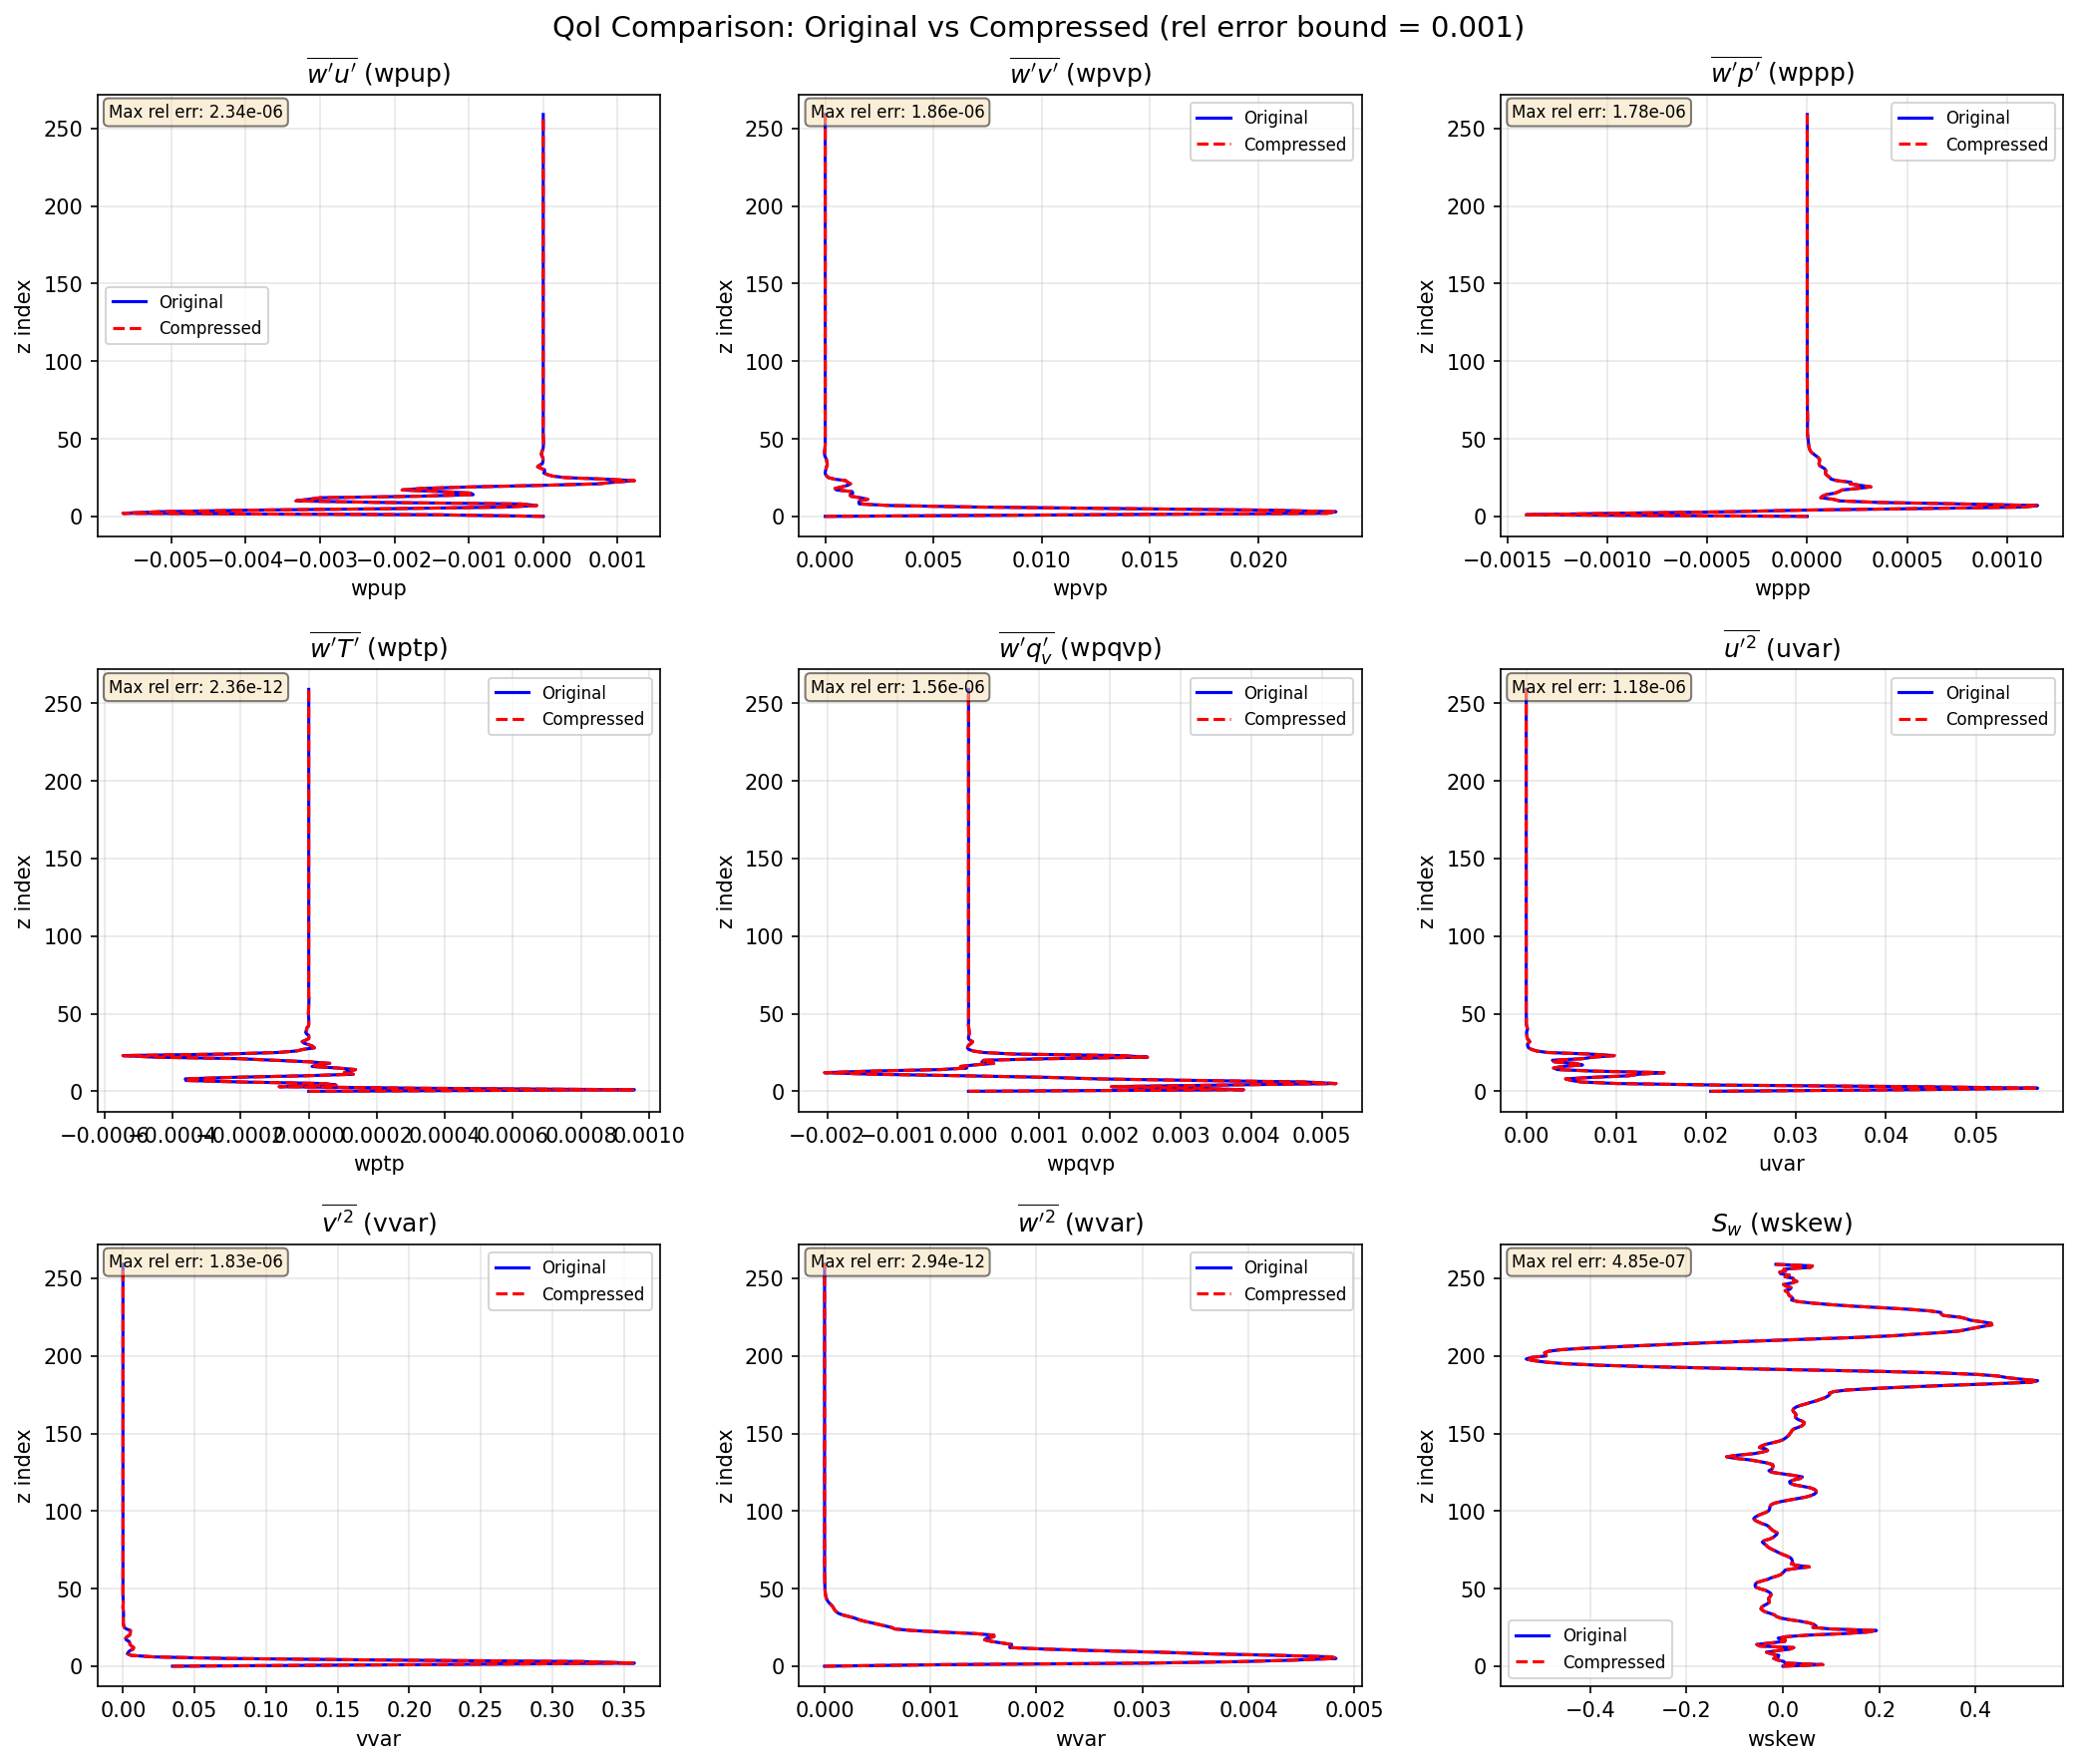
\includegraphics[width=\textwidth]{qoi_comparison.png}
\caption{Comparison of 9 QoIs computed from original data vs. compressed/decompressed data (relative error bound = $10^{-3}$). Each QoI is a 1D profile of length $N_z = 260$. Blue: original, Red dashed: compressed. All QoIs from original data and compressed data are almost identical, which indicates over conservative errror bounds}
\end{figure}


%==============================================================================
\section{Empirical Per-Field Bound Search}
%==============================================================================

The analytical QPET bounds derived above are conservative: the first-order
Taylor propagation over-bounds $W$ (driving $\epsilon_W$ to $\sim 10^{-9}$) and
limits the overall ratio. We therefore introduce an \emph{empirical} per-field
search that finds, for each field, the loosest absolute error bound that still
keeps every dependent QoI within its target, by directly compressing,
decompressing, and measuring the resulting QoI error. The framework is
compressor-agnostic and is evaluated with three error-bounded compressors:
SZ3, zfp, and SPERR.

\subsection{QoI Error Metric}

For each QoI we use the range-relative maximum error over the vertical profile:
\begin{equation}
  E(\text{QoI}) = \frac{\max_z \lvert \text{QoI}_{\text{orig}}(z) -
  \text{QoI}_{\text{dec}}(z)\rvert}{\max_z \text{QoI}_{\text{orig}}(z) -
  \min_z \text{QoI}_{\text{orig}}(z)} \le \tau,
\end{equation}
where $\tau$ is the target relative QoI bound, applied uniformly to all nine QoIs.

\subsection{Per-Field Binary Search}

For a single field, the highest admissible bound is found by \textbf{binary
search} over the absolute error bound $\epsilon$ in logarithmic space on
$[\,r\cdot 10^{-7},\; r\cdot 0.5\,]$, where $r$ is the field's value range. At
each step the field is compressed and decompressed at the trial $\epsilon$, the
dependent QoI(s) are recomputed, and the trial passes iff all satisfy
$E \le \tau$. If the midpoint passes, the floor is raised (looser bound);
otherwise the ceiling is lowered (tighter bound). The largest passing bound,
scaled by a safety margin ($0.9$), is returned. The iteration count is capped to
limit the impact of compressor non-monotonicity.

\subsection{QoI Search Sequence}

A key property is \textbf{separability}: because each perturbation subtracts a
per-field horizontal mean, a QoI depends only on its own field(s); compressing
field $A$ never alters a QoI that does not depend on $A$. A per-field search with
the coupled field(s) fixed therefore reproduces the all-fields result exactly.
Since $W$ appears in all nine QoIs but is constrained by single-field QoIs only
($wvar$, $wskew$), it is locked first:
\begin{enumerate}
  \item \textbf{Phase 1 (single-field QoIs).} Search $U$ via $uvar$, $V$ via
  $vvar$, and $W$ via both $wvar$ and $wskew$ (the tighter bound wins). Fix $W$
  at its decompressed array for the next phase.
  \item \textbf{Phase 2 (multi-field QoIs, $W$ fixed).} Search $PP$ via $wppp$,
  $TABS$ via $wptp$, and $QV$ via $wpqvp$; re-search $U$ via $wpup$ and $V$ via
  $wpvp$. Each field's final bound is the minimum of its Phase-1 and Phase-2
  results.
\end{enumerate}
This is the same dependency-ordered sequence motivated in the analytical method,
but the bounds are determined empirically rather than via Taylor formulas.

\subsection{$W$-Coupling Fallback}

If a bilinear QoI cannot be met even with its partner field near-lossless --- i.e.
$W$'s own error already exhausts the QoI budget --- $W$ is tightened and Phase 2
is restarted. Tightening $W$ only improves every other QoI, so the step is always
safe.

\subsection{Final Verification and Tightening}

After the per-field bounds are fixed, all six fields are compressed
simultaneously and all nine QoIs are recomputed. Should any QoI marginally exceed
its target --- possible because of compressor non-monotonicity and the shared $W$
coupling --- the bounds of the fields feeding that QoI are \textbf{tightened} by a
factor of $0.9$ and the verification is repeated, for a small bounded number of
rounds.

\subsection{Lossless Fallback}

A QoI that remains infeasible even with its fields near-lossless triggers
\textbf{lossless} storage of those fields. In practice this affects only $W$,
driven by $wskew$: the normalized third moment is hypersensitive to error at
low-variance heights, so some compressors cannot bound it at any lossy setting.
Lossless storage uses each backend's native mode (zfp reversible, SZ3 with error
bound $0$) and falls back to raw storage where there is none (SPERR). Such fields
are reported with bound $0$.

%==============================================================================
\section{Multi-Compressor Results}
%==============================================================================

We run nine configurations: three compressors (SZ3, zfp, SPERR) at three
relative QoI bounds ($10^{-2}$, $10^{-3}$, $10^{-4}$), each applied uniformly to
all nine QoIs, on a single timestep (six \texttt{float32} fields,
$408.9$\,MB total). Every configuration satisfies all nine QoIs, using the
lossless fallback where noted. Table~\ref{tab:overall} reports the overall ratio,
Figure~\ref{fig:perfield-hist} and Table~\ref{tab:perfield-ratio} the per-field
ratio, Table~\ref{tab:perfield-eb} the per-field error bounds, and
Table~\ref{tab:full} the full per-configuration detail.

\begin{table}[H]
\centering
\caption{Overall compression ratio for all nine configurations.}
\label{tab:overall}
\begin{tabular}{lccc}
\toprule
\textbf{Compressor} & $\tau=10^{-2}$ & $\tau=10^{-3}$ & $\tau=10^{-4}$ \\
\midrule
SZ3 & 30.52x & 18.30x & 10.87x \\
zfp & 6.23x & 5.68x & 5.09x \\
SPERR & 15.80x & 13.47x & 5.13x \\
\bottomrule
\end{tabular}
\end{table}

\begin{figure}[H]
\centering
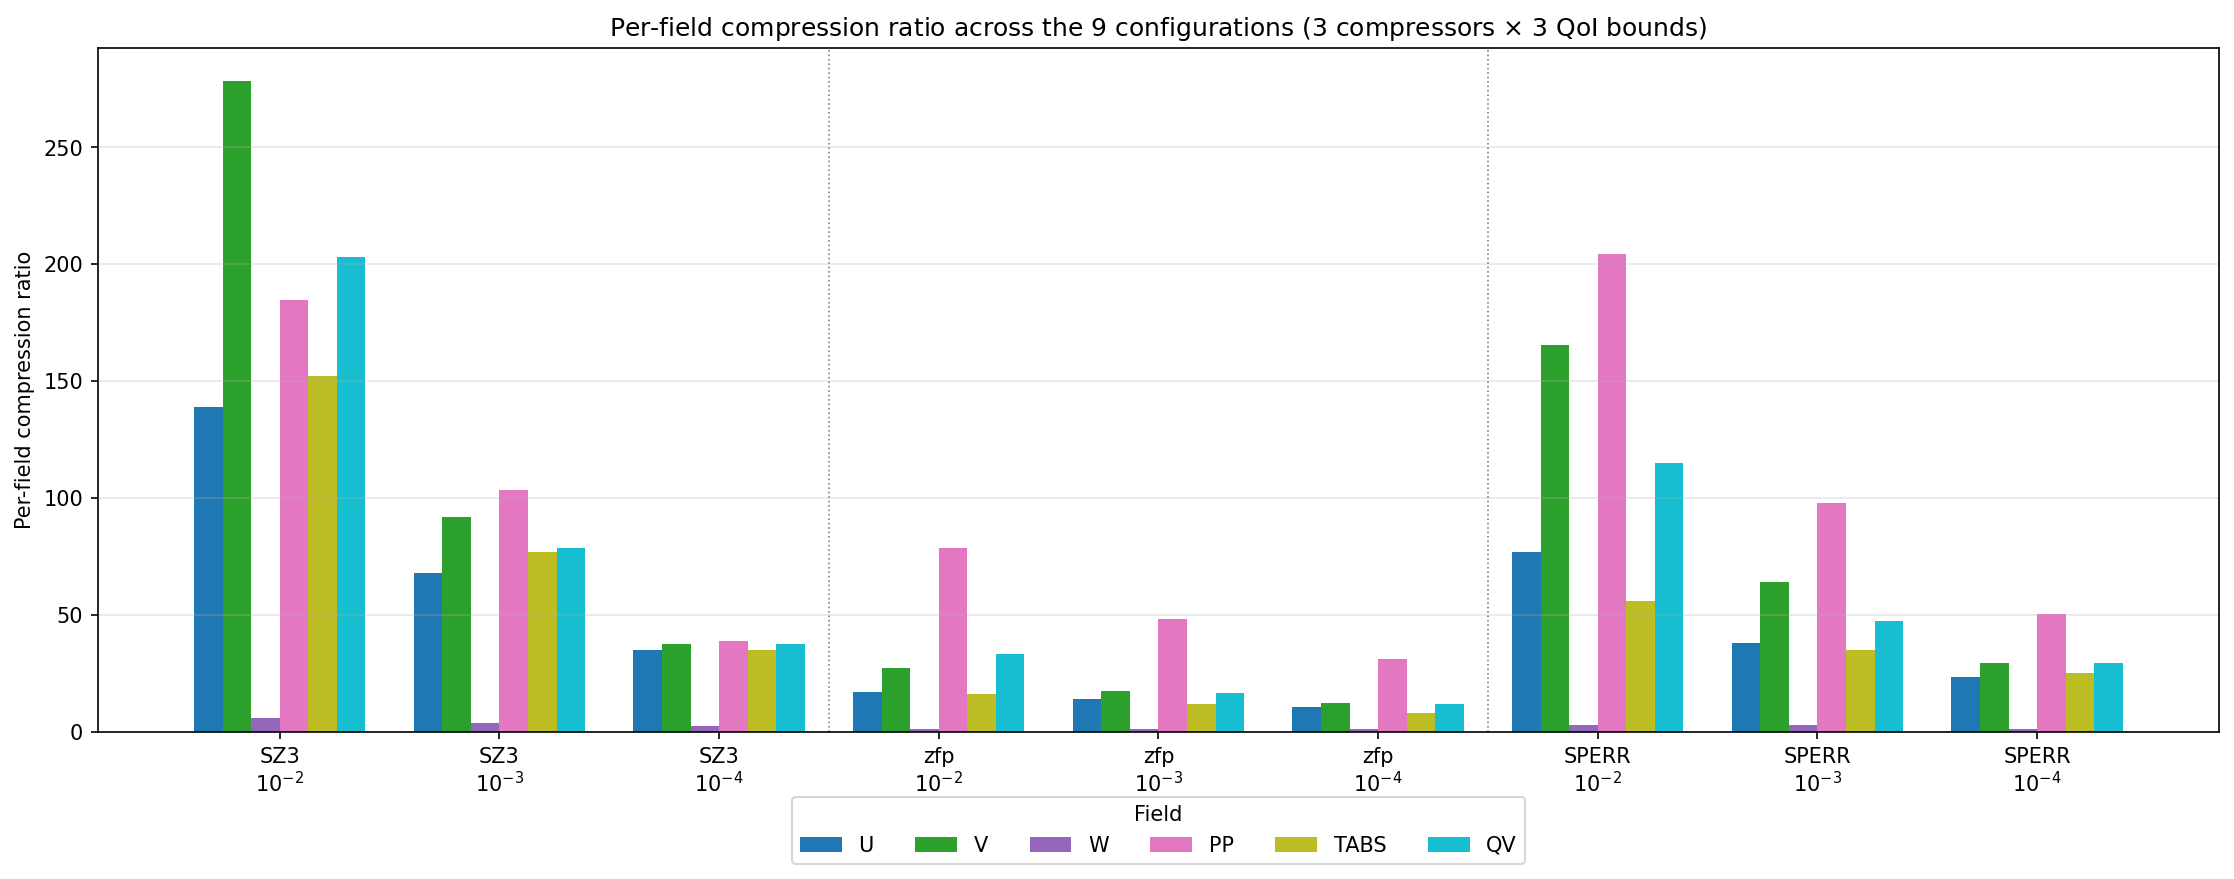
\includegraphics[width=\textwidth]{perfield_ratio_hist.png}
\caption{Per-field compression ratio for the nine configurations. Each cluster
is one configuration (compressor at a given QoI bound) and contains one column
per field ($U, V, W, PP, TABS, QV$). Dotted lines separate the three
compressors.}
\label{fig:perfield-hist}
\end{figure}

\begin{table}[H]
\centering
\caption{Per-field compression ratio across all nine configurations.}
\label{tab:perfield-ratio}
\resizebox{\textwidth}{!}{%
\begin{tabular}{l ccc ccc ccc}
\toprule
& \multicolumn{3}{c}{SZ3} & \multicolumn{3}{c}{zfp} & \multicolumn{3}{c}{SPERR} \\
\cmidrule(lr){2-4}\cmidrule(lr){5-7}\cmidrule(lr){8-10}
\textbf{Field} & $10^{-2}$ & $10^{-3}$ & $10^{-4}$ & $10^{-2}$ & $10^{-3}$ & $10^{-4}$ & $10^{-2}$ & $10^{-3}$ & $10^{-4}$ \\
\midrule
U & 138.89x & 68.11x & 35.10x & 17.16x & 14.23x & 10.49x & 76.73x & 37.88x & 23.38x \\
V & 278.43x & 92.07x & 37.42x & 27.18x & 17.45x & 12.30x & 165.33x & 64.07x & 29.24x \\
W & 5.92x & 3.75x & 2.41x & 1.31x & 1.31x & 1.31x & 3.04x & 2.91x & 1.00x \\
PP & 184.59x & 103.36x & 38.78x & 78.70x & 48.36x & 30.97x & 204.24x & 97.92x & 50.51x \\
TABS & 152.21x & 77.01x & 34.85x & 16.18x & 11.90x & 8.20x & 56.15x & 35.00x & 25.00x \\
QV & 203.23x & 78.57x & 37.35x & 33.19x & 16.41x & 11.72x & 114.86x & 47.21x & 29.48x \\
\midrule
\textbf{Overall} & \textbf{30.52x} & \textbf{18.30x} & \textbf{10.87x} & \textbf{6.23x} & \textbf{5.68x} & \textbf{5.09x} & \textbf{15.80x} & \textbf{13.47x} & \textbf{5.13x} \\
\bottomrule
\end{tabular}}
\end{table}

\begin{table}[H]
\centering
\caption{Per-field relative error bound found by the search across all nine configurations. ``lossless denotes a field stored without loss.}
\label{tab:perfield-eb}
\resizebox{\textwidth}{!}{%
\begin{tabular}{l ccc ccc ccc}
\toprule
& \multicolumn{3}{c}{SZ3} & \multicolumn{3}{c}{zfp} & \multicolumn{3}{c}{SPERR} \\
\cmidrule(lr){2-4}\cmidrule(lr){5-7}\cmidrule(lr){8-10}
\textbf{Field} & $10^{-2}$ & $10^{-3}$ & $10^{-4}$ & $10^{-2}$ & $10^{-3}$ & $10^{-4}$ & $10^{-2}$ & $10^{-3}$ & $10^{-4}$ \\
\midrule
U & \num{1.61e-03} & \num{4.97e-04} & \num{1.14e-04} & \num{2.86e-02} & \num{1.43e-02} & \num{3.57e-03} & \num{3.19e-03} & \num{7.39e-04} & \num{1.54e-04} \\
V & \num{3.70e-03} & \num{1.04e-03} & \num{2.07e-04} & \num{9.68e-02} & \num{2.42e-02} & \num{6.05e-03} & \num{5.82e-03} & \num{1.67e-03} & \num{2.61e-04} \\
W & \num{4.13e-06} & \num{5.85e-07} & \num{6.56e-08} & lossless & lossless & lossless & \num{9.00e-08} & \num{6.56e-08} & lossless \\
PP & \num{4.90e-03} & \num{1.99e-03} & \num{2.97e-04} & \num{1.44e-01} & \num{3.61e-02} & \num{9.02e-03} & \num{6.11e-03} & \num{1.48e-03} & \num{2.93e-04} \\
TABS & \num{8.65e-05} & \num{3.12e-05} & \num{6.89e-06} & \num{4.77e-03} & \num{1.19e-03} & \num{1.49e-04} & \num{1.44e-04} & \num{4.23e-05} & \num{1.30e-05} \\
QV & \num{2.54e-03} & \num{4.78e-04} & \num{8.92e-05} & \num{1.14e-01} & \num{1.42e-02} & \num{3.56e-03} & \num{4.01e-03} & \num{7.15e-04} & \num{2.00e-04} \\
\bottomrule
\end{tabular}}
\end{table}

{\footnotesize
\begin{longtable}{lccc}
\caption{Full per-configuration detail: per-field absolute bound, relative bound, and compression ratio for every field in all nine configurations. Fields stored losslessly are shown with bound 0.}\label{tab:full}\\
\toprule
\textbf{Field} & \textbf{Abs. bound} & \textbf{Rel. bound} & \textbf{Ratio} \\ \midrule
\endfirsthead
\multicolumn{4}{l}{\emph{(continued)}}\\ \toprule
\textbf{Field} & \textbf{Abs. bound} & \textbf{Rel. bound} & \textbf{Ratio} \\ \midrule
\endhead
\bottomrule
\endfoot
\multicolumn{4}{l}{\textbf{SZ3, $\tau=10^{-2}$ --- overall 30.52x}}\\
\midrule
U & \num{2.542e-02} & \num{1.614e-03} & 138.89x \\
V & \num{6.878e-02} & \num{3.698e-03} & 278.43x \\
W & \num{2.391e-06} & \num{4.129e-06} & 5.92x \\
PP & \num{7.642e-03} & \num{4.899e-03} & 184.59x \\
TABS & \num{4.081e-03} & \num{8.646e-05} & 152.21x \\
QV & \num{2.006e-02} & \num{2.536e-03} & 203.23x \\
\midrule
\addlinespace
\multicolumn{4}{l}{\textbf{SZ3, $\tau=10^{-3}$ --- overall 18.30x}}\\
\midrule
U & \num{7.824e-03} & \num{4.967e-04} & 68.11x \\
V & \num{1.937e-02} & \num{1.042e-03} & 92.07x \\
W & \num{3.387e-07} & \num{5.850e-07} & 3.75x \\
PP & \num{3.100e-03} & \num{1.987e-03} & 103.36x \\
TABS & \num{1.475e-03} & \num{3.124e-05} & 77.01x \\
QV & \num{3.783e-03} & \num{4.783e-04} & 78.57x \\
\midrule
\addlinespace
\multicolumn{4}{l}{\textbf{SZ3, $\tau=10^{-4}$ --- overall 10.87x}}\\
\midrule
U & \num{1.793e-03} & \num{1.138e-04} & 35.10x \\
V & \num{3.846e-03} & \num{2.068e-04} & 37.42x \\
W & \num{3.799e-08} & \num{6.561e-08} & 2.41x \\
PP & \num{4.633e-04} & \num{2.970e-04} & 38.78x \\
TABS & \num{3.252e-04} & \num{6.890e-06} & 34.85x \\
QV & \num{7.057e-04} & \num{8.922e-05} & 37.35x \\
\midrule
\addlinespace
\multicolumn{4}{l}{\textbf{zfp, $\tau=10^{-2}$ --- overall 6.23x}}\\
\midrule
U & \num{4.500e-01} & \num{2.857e-02} & 17.16x \\
V & \num{1.800e+00} & \num{9.679e-02} & 27.18x \\
W & 0 & 0 & 1.31x \\
PP & \num{2.250e-01} & \num{1.442e-01} & 78.70x \\
TABS & \num{2.250e-01} & \num{4.766e-03} & 16.18x \\
QV & \num{9.000e-01} & \num{1.138e-01} & 33.19x \\
\midrule
\addlinespace
\multicolumn{4}{l}{\textbf{zfp, $\tau=10^{-3}$ --- overall 5.68x}}\\
\midrule
U & \num{2.250e-01} & \num{1.428e-02} & 14.23x \\
V & \num{4.500e-01} & \num{2.420e-02} & 17.45x \\
W & 0 & 0 & 1.31x \\
PP & \num{5.625e-02} & \num{3.606e-02} & 48.36x \\
TABS & \num{5.625e-02} & \num{1.192e-03} & 11.90x \\
QV & \num{1.125e-01} & \num{1.422e-02} & 16.41x \\
\midrule
\addlinespace
\multicolumn{4}{l}{\textbf{zfp, $\tau=10^{-4}$ --- overall 5.09x}}\\
\midrule
U & \num{5.625e-02} & \num{3.571e-03} & 10.49x \\
V & \num{1.125e-01} & \num{6.049e-03} & 12.30x \\
W & 0 & 0 & 1.31x \\
PP & \num{1.406e-02} & \num{9.015e-03} & 30.97x \\
TABS & \num{7.031e-03} & \num{1.490e-04} & 8.20x \\
QV & \num{2.812e-02} & \num{3.556e-03} & 11.72x \\
\midrule
\addlinespace
\multicolumn{4}{l}{\textbf{SPERR, $\tau=10^{-2}$ --- overall 15.80x}}\\
\midrule
U & \num{5.032e-02} & \num{3.194e-03} & 76.73x \\
V & \num{1.082e-01} & \num{5.820e-03} & 165.33x \\
W & \num{5.212e-08} & \num{9.000e-08} & 3.04x \\
PP & \num{9.536e-03} & \num{6.114e-03} & 204.24x \\
TABS & \num{6.800e-03} & \num{1.441e-04} & 56.15x \\
QV & \num{3.171e-02} & \num{4.009e-03} & 114.86x \\
\midrule
\addlinespace
\multicolumn{4}{l}{\textbf{SPERR, $\tau=10^{-3}$ --- overall 13.47x}}\\
\midrule
U & \num{1.164e-02} & \num{7.392e-04} & 37.88x \\
V & \num{3.111e-02} & \num{1.673e-03} & 64.07x \\
W & \num{3.799e-08} & \num{6.561e-08} & 2.91x \\
PP & \num{2.313e-03} & \num{1.483e-03} & 97.92x \\
TABS & \num{1.997e-03} & \num{4.231e-05} & 35.00x \\
QV & \num{5.658e-03} & \num{7.152e-04} & 47.21x \\
\midrule
\addlinespace
\multicolumn{4}{l}{\textbf{SPERR, $\tau=10^{-4}$ --- overall 5.13x}}\\
\midrule
U & \num{2.434e-03} & \num{1.545e-04} & 23.38x \\
V & \num{4.858e-03} & \num{2.612e-04} & 29.24x \\
W & 0 & 0 & 1.00x \\
PP & \num{4.574e-04} & \num{2.933e-04} & 50.51x \\
TABS & \num{6.124e-04} & \num{1.297e-05} & 25.00x \\
QV & \num{1.578e-03} & \num{1.995e-04} & 29.48x \\
\midrule
\end{longtable}
}


\textcolor{red}{\textbf{Takeaway:} SZ3 gives the best QoI-preserving compression
at every bound ($30.5\times$ / $18.3\times$ / $10.9\times$) --- about $2\times$
SPERR and $3$--$5\times$ zfp --- and is the only compressor that preserves
$wskew$ without storing $W$ losslessly. SPERR is competitive only at the looser
bounds and collapses at $10^{-4}$ (raw $W$, as it has no lossless mode), while
zfp is weakest throughout and must store $W$ losslessly at every bound.}

\textcolor{red}{\textbf{Takeaway:} $W$ is the universal bottleneck: the skewness
$wskew$ forces its error bound roughly three orders of magnitude tighter than any
other field, and every lossless fallback in this study is $W$. Preserving
vertical-velocity skewness is what caps the overall compression ratio.}


\end{document}
